\section{Thiết kế API}

Hệ thống giao diện lập trình ứng dụng (API) của \textit{Secret Letter} được thiết kế theo tiêu chuẩn RESTful, đảm nhiệm vai trò cầu nối duy nhất giữa máy khách (Frontend) và bộ xử lý lưu trữ (Backend). Khác với các kiến trúc CRUD thông thường, lớp API này chịu trách nhiệm hỗ trợ thực thi các chính sách bảo mật biên (Edge Security) và quản lý vòng đời tiêu thụ dữ liệu một lần (One-time Reveal).

\subsection{Cấu trúc Middleware và Kiểm duyệt biên}

Để thu hẹp các bề mặt tấn công từ lớp mạng, các luồng dữ liệu HTTP trước khi chạm đến các bộ xử lý logic (Handlers) được yêu cầu đi qua một chuỗi Middleware phòng thủ theo chiều sâu (Defense in Depth). Kiến trúc này được định nghĩa trực tiếp tại mã nguồn \texttt{internal/\-httpapi/\-server.go}:

\begin{figure}[H]
\centering
\begin{tikzpicture}[
    font=\sffamily\small,
    >={Stealth[round, scale=1.1]},
    client/.style={draw=orange!40, fill=orange!5, rounded corners=6pt, inner sep=8pt, align=center, font=\bfseries},
    middleware/.style={draw=blue!30, fill=blue!5, rounded corners=6pt, inner sep=6pt, align=center, minimum width=4.5cm, minimum height=0.8cm},
    handler/.style={draw=purple!40, fill=purple!5, rounded corners=6pt, inner sep=8pt, align=center, minimum width=2.5cm},
    arrow/.style={->, thick, gray!80, rounded corners=4pt}
]

\node[client] (client) at (0, 6) {Client Request};
\node[middleware] (mw1) at (0, 4.5) {Rate Limiting (IP Bucket)};
\node[middleware] (mw2) at (0, 3.2) {Request Size Limit (15KB)};
\node[middleware] (mw3) at (0, 1.9) {Security Headers \& CORS};
\node[middleware] (mw4) at (0, 0.6) {Structured Logging (SHA-256 IP)};

\node[handler] (h1) at (-3.8, -1.5) {POST\\/api/secrets};
\node[handler] (h2) at (0, -1.5) {POST\\/api/reveal-sessions};
\node[handler] (h3) at (3.8, -1.5) {POST\\/api/secrets/:id/open};

\draw[arrow] (client) -- (mw1);
\draw[arrow] (mw1) -- (mw2);
\draw[arrow] (mw2) -- (mw3);
\draw[arrow] (mw3) -- (mw4);
\draw[arrow] (mw4) -- (h1);
\draw[arrow] (mw4) -- (h2);
\draw[arrow] (mw4) -- (h3);

\end{tikzpicture}
\caption{Luồng xử lý yêu cầu đi qua hệ thống Middleware của API Gateway}
\label{fig:api_middleware_flow}
\end{figure}

Việc áp dụng các khối Middleware mang lại giá trị bảo mật hiện hữu:
\begin{itemize}
    \item \textbf{withRequestSizeLimit}: Hỗ trợ ngắt kết nối thông qua \texttt{http.\-MaxBytesReader} nếu tải trọng (Payload) vượt ngưỡng \texttt{15KB}, giúp ngăn chặn nguy cơ tấn công bơm rác làm tràn bộ nhớ (Data Flooding).
    \item \textbf{withSecurityHeaders}: Áp dụng các tiêu đề phản hồi bảo mật nhằm hạn chế rủi ro từ trình duyệt, bao gồm \texttt{Strict-Transport-Security (HSTS)} để yêu cầu dùng HTTPS, \texttt{X-Content-Type-Options: nosniff} chống đánh lừa định dạng, và \texttt{Content-Security-Policy (CSP)} nhằm kiểm soát nguồn thực thi mã.
    \item \textbf{withRequestLogging}: Bảo vệ quyền riêng tư bằng cách băm (hash) địa chỉ IP gốc và \texttt{User-Agent} bằng thuật toán SHA-256 trước khi xuất ra hệ thống Log nội bộ, đồng thời gắn kèm \texttt{X-Request-ID} dạng UUID để hỗ trợ truy vết.
\end{itemize}

\subsection{Đặc tả Endpoints cốt lõi}

Tài nguyên API được chia thành ba luồng thao tác bất biến, phản ánh vòng đời của một \textit{Secret}:

\subsubsection{Khởi tạo Thông điệp mã hóa}
Giao thức này tiếp nhận bản mã (ciphertext) đã được sinh ra tại trình duyệt và tiến hành lưu trữ vào In-Memory Database.
\begin{itemize}
    \item \textbf{Method \& Path:} \texttt{POST /api/secrets}
    \item \textbf{Headers bắt buộc:} \texttt{Content-Type: application/json}
    \item \textbf{Body Input:} Chứa các thuộc tính đã mã hóa bao gồm \texttt{ciphertext} (Bản mã Base64URL), \texttt{nonce} (IV khởi tạo ngẫu nhiên), \texttt{algorithm} (chuẩn thuật toán, mặc định là AES-GCM), và \texttt{ttlSeconds} (thời gian sống tính bằng giây).
    \item \textbf{Response Thành công (201 Created):} Trả về ID định danh nội bộ (\texttt{secretId}) và thời điểm sẽ bị tiêu hủy tự động (\texttt{expiresAt}).
    \item \textbf{Response Lỗi (4xx):} Trả về mã \texttt{413 Payload Too Large} nếu cấu trúc JSON vượt 15KB, hoặc mã \texttt{400 Validation Failed} nếu Request thiếu trường thông tin hợp lệ.
\end{itemize}

\subsubsection{Cơ chế Anti-Bot và Phiên giải mã (Reveal Session)}
Là cơ chế hỗ trợ ngăn ngừa các công cụ xem trước (Preview Bots) như Zalo, Telegram, Discord tự động tiêu thụ liên kết bí mật.
\begin{itemize}
    \item \textbf{Method \& Path:} \texttt{POST /api/reveal-sessions}
    \item \textbf{Vận hành:} Khi người nhận truy cập lần đầu tiên, giao diện sẽ gửi yêu cầu cấp một phiên làm việc (Session) ngắn hạn gắn với \texttt{secretId} đó. Thao tác này là bằng chứng xác thực có một người dùng thực sự đang chờ bấm nút "Mở thư".
    \item \textbf{Response (201 Created):} Cấp phát mã \texttt{sessionId} tạm thời để sử dụng cho bước tiếp theo.
\end{itemize}

\subsubsection{Truy vấn Trạng thái và Tiêu thụ (Consume)}
Hai API này đảm nhận khâu cuối cùng trong vòng đời thông điệp. Điểm đặc biệt của toàn bộ nhóm API \texttt{/secrets/:id/*} là máy chủ sẽ chủ động chèn thêm Header \texttt{Cache-Control: no-store} nhằm hạn chế tình trạng trình duyệt tải lại nội dung cũ đã bị xóa.
\begin{itemize}
    \item \textbf{\texttt{GET /api/secrets/:id/status}:} Trả về trạng thái hiện hành của thư (\texttt{active}, \texttt{consumed}, \texttt{expired}, \texttt{not\_found}) nhưng không thực thi việc xóa. Dùng để render giao diện kiểm tra.
    \item \textbf{\texttt{POST /api/secrets/:id/open} (hoặc \texttt{/consume}):} Kích hoạt chuỗi lệnh Lua Script nguyên tử trên Redis để trả về nguyên trạng bản mã, và ngay lập tức thực thi lệnh xóa sổ (DEL) bản ghi. Yêu cầu truyền vào Header \texttt{X-Reveal-Session} từ bước số 2 để chứng thực tính hợp lệ. Giao dịch thành công trả về \texttt{200 OK} kèm dữ liệu; nếu thất bại do thư đã bốc hơi, trả về \texttt{410 Gone} kèm thông báo chuẩn hóa.
\end{itemize}

\subsection{Vòng đời Thông điệp (Secret Lifecycle)}

Sự tương tác giữa các API nói trên cấu thành một vòng đời dữ liệu khép kín (như minh họa tại Hình \ref{fig:api_state_lifecycle}).

Việc định nghĩa rõ ràng các trạng thái (\texttt{active}, \texttt{consumed}, \texttt{expired}, \texttt{not\_found}) giúp hệ thống phản ứng linh hoạt trước các tình huống thực tế. Đặc biệt, thao tác tiêu hủy được thiết kế để thi hành ngay lập tức (Atomic DEL) khi người dùng mở thư, hoặc được hệ thống tự động dọn dẹp bởi cơ chế Key Eviction của Redis khi cạn thời gian sống (TTL). Điều này đóng vai trò quyết định trong việc duy trì nguyên lý "chỉ đọc một lần" (Burn-after-reading) của dự án.

\begin{figure}[H]
    \centering
    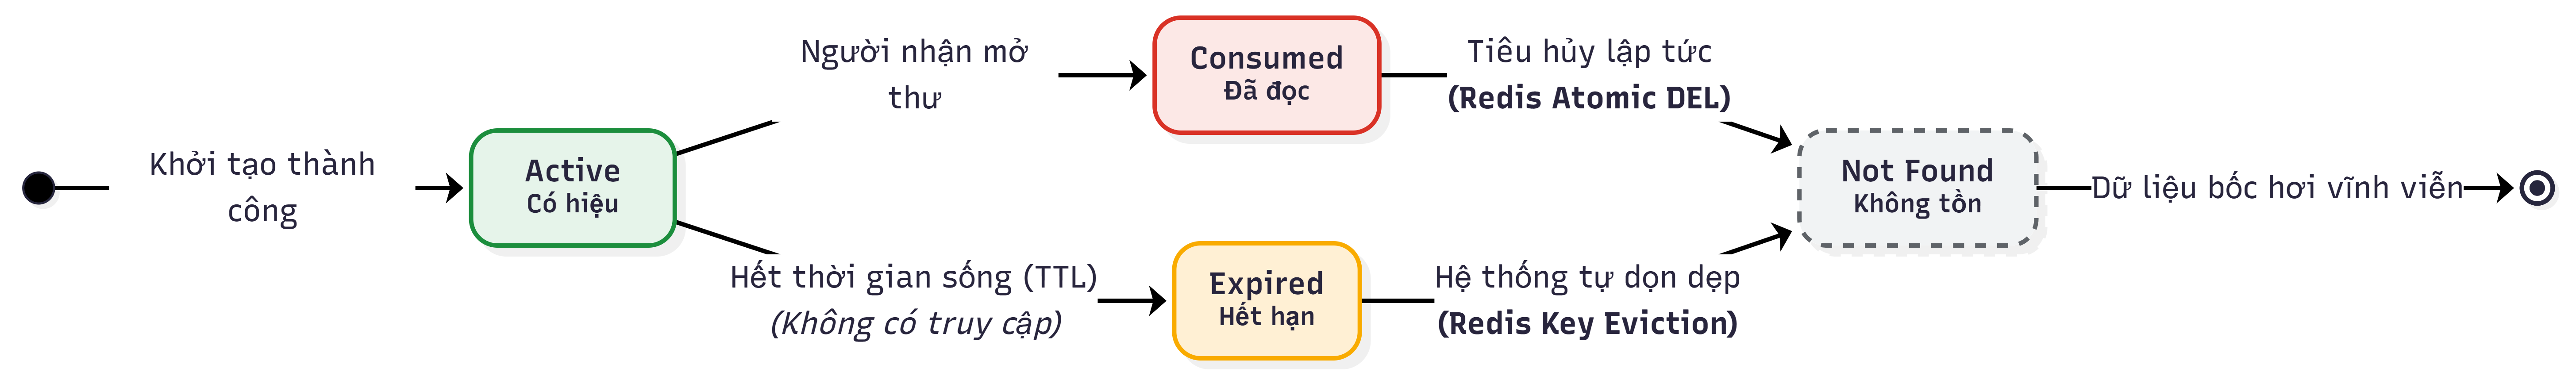
\includegraphics[width=1.0\textwidth]{img/state_lifecycle.png}
    \caption{Sơ đồ trạng thái minh họa vòng đời lưu trữ của một thông điệp}
    \label{fig:api_state_lifecycle}
\end{figure}

\subsection{Tiêu chuẩn hóa Quản lý lỗi (Error Handling)}
Các phản hồi lỗi từ API được thiết kế để không trả về chuỗi văn bản thuần (raw string). Thay vào đó, bộ Middleware của Backend trừu tượng hóa các lỗi này thành cấu trúc \texttt{AppError} chuẩn hóa. Khối JSON lỗi mang định dạng \texttt{\{"code": "...", "message": "...", "details": \{...\}\}}. Cách tiếp cận này (nhất quán trong toàn bộ \texttt{handlers.go}) giúp quy trình xử lý trên Frontend trở nên thuận tiện hơn, hỗ trợ ánh xạ logic hiển thị lỗi (Error Boundary UI) một cách rõ ràng theo từng mã định danh cục bộ.